\documentclass[11pt]{article}
\setlength{\textheight}{210mm}
\addtolength{\topmargin}{-15mm}
\setlength{\textwidth}{155mm}
\setlength{\oddsidemargin}{5mm}
\usepackage{graphicx, subcaption, amsfonts}
\graphicspath{ {./figs/} }
\pagestyle{plain}
\begin{document}
\title{Dynamics of networks: generation, dimensionality reduction, and coarse-grained evolution of graphs}
\author{\LARGE Proposed by Alexander Holiday\vspace{3mm}\\\Large under the supervision of\vspace{3mm}\\\LARGE Professor Yannis Kevrekidis}
\date{11/01/2013}
\maketitle

\begin{figure}[h]
  \centering
  
\includegraphics[width=0.5\textwidth]{princeton_shield}
\end{figure}

\clearpage

\section{Introduction}

From collaborations among movie stars \cite{barbasi} to gene interactions in \texit{C. elegans}\cite{harvardCelegans}, network science has found a vast array of applications in the past two decades. This is largely a result of the generality of the network framework: myriad systems are readily adapted to such a description; interacting bodies (e.g. a city, person, or protein) form nodes in the network, the connections between them (e.g. via highways, Facebook friendships, or biological suppresion) create edges. Thus, one may usefully apply the same abstraction to study such disparate topics as the spread of opinions in a society and chemical reaction networks. \vspace{1mm}\\
However, too often this merely leads to a recasting of the original problem. While this, in itself, can be useful, it fails to exploit the true power in such a formulation. Several obstacles prevent this full realization, a selection of which will be the focus of this proposal. Broadly speaking, the generality of the construct is in some sense its undoing: while numerous problems are addressable, they require many different types of analysis. Thus, a researcher in neural networks may use none of the same tools as a civil engineer designing tranporation networks. Certainly, the dynamics between proteins in a cell and drivers in rush-hour traffic may share almost no similarities; however, this should not prevent investigators in these fields from having similar analytical tools at their disposal.\vspace{1mm}\\ %missing something on dynamics ``of'' and not ``on'', why study ``of''?
One of these tools may be considered a foundation upon which all others rest: the ability to computationally construct networks with desired properties. There are several examples in which, during the course of analysis of a system, incorrect conclusions were drawn due to improper modeling of the network architecture itself \cite{theinternetisscalefree,smallworld,etc.}. For instance, early network research into the internet tended to model its structure in the following, simple manner: each webpage (a node of the network), was randomly connected to each other webpage with some given probability $p$ (creating what is known as an Erd\H{o}s-R\'{e}nyi random graph, detailed below) \cite{stochastic_models_webgraph}. The simple structure lent itself to easier calculations, but as future papers emerged detailing the Web's actual structure, these early results were dismissed \cite{something,hopefully}. As the intimate link between a network's underlying structure and its resulting dynamics becomes increasingly evident \cite{barbasi,scalefree and/or barabasi global dynamics}, it becomes difficult to justify the use of simple models in lieu of the ability to construct more accurate versions (or, at the very least, one cannot fully trust any subsequent results). Unfortunately, there is currently a lack of methods available to researchers for the construction of networks with desired properties. The algorithms that do exist tend to address a single network variable (e.g. the average number of connections a node has), leaving others unspecified. In fact, in collaboration with the Floudas lab, a general network generation method capable of simultaneously stipulating multiple properties has recently been developed; but, while a very promising step forward, the scalability of the approach must be improved if large systems are to be created \cite{karthiksoptimizationpaper}. Therefore, there remains a need for a general algorithm capable of generating a network with arbitrary specifications.\vspace{1mm}\\
Even if one succeeds in accurately modeling a network's structure, the resulting data can be unwieldly and overwhelming. Consider a simple example: the religious affiliation of Facebook members. Our data consists of a list of all Facebook users, the links between them (``friendships''), and the declared religion of each member (let us assume everyone makes such information public). Given this information, a seemingly benign question might be: what is the driving factor in an individual's religious association. Initially, reasoning that those with many friends of a certain relgion will tend to follow suit, one might correlate religion with the fraction of friends who share the same. However, it could also be reasoned that children tend to align themselves similarly with their parents. Studying this effect in isolation is feasible, but a method of combining this effect with that of the individuals friends isn't obvious. Perhaps, too, there are certain highly connected individuals who vocally advocate their religion, causing many of their friends to convert (e.g. pastors, rabbis, imams, etc.). Here, even the proper identification of such individuals is unclear. We have a static data set, in which only one property has been measured at each node, yet there are many possible methods of analysis (some easier than others), each potentially leading to very different conclusions. Considering most data sets evolve in time (are dynamic) and many specify more than one property at each node, a suite of generalized methods for mining data from networks would be a great help in guiding research efforts. \vspace{1mm}\\
This is not a new problem, but while a host of network diagnostics exist (for examples, see \cite{diffusion distances} \cite{clustering}), there remains much room for improvement. A popular method of community detection (grouping like nodes) is currently ``modularity''. This has been successfully applied to several systems (\cite{basset} \cite{more bassett}), but its usefullness hinges on the knowledge of an appropriate ``null network'' for the system. Other methods require the specification of certain algorithmic constants whose relevance to the underlying problem is unclear. For example, algorithms based on random walks often leave the maximum length of the walk, the initial distribution of walkers, and the stopping probabilities as parameters \cite{japan_ibm_graph_kernels}. There is no generic procedure for specifying these values for a given system. 
\begin{figure}[h!]
  \centering
  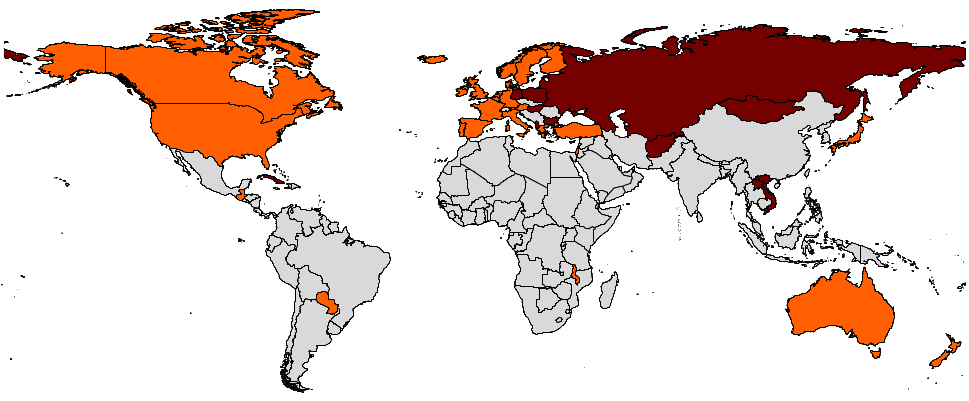
\includegraphics[width=10cm]{unCommunityDetection}
  \caption{Grouping of countries based on United Nations voting records using the modularity method \cite{porter}.}
  \label{fig:un}
\end{figure}
\vspace{1mm}\\
Many of these techniques constitute research areas in their own right: community detection, node-node similarity and pattern recognition each have several dedicated algorithms \cite{laZagerMIT} \cite{kleinberg} \cite{modularity} \cite{neuralnetwork pattern recog}. However, they aim to mine data from a single network. An avenue that has received relatively little attention, and one especially relevant to the study of dynamic systems, is formulating techniques that operate \texit{across} networks. Extracting information from a set of networks presents special challenges, but as the number of temporally-resolvable systems increases, so, too, does the importance of such an ability. While we focus on this aspect, data mining among networks, it should be noted that the previous discussion of single-network diagnostics was not in vain as they may be adaptable to operate on this added dimension. Indeed, initial research in this topic will concentrate on modifying such existing methods. \vspace{1mm}\\
Finally, combining the ability to create specific networks on demand with methods for determining important network characteristics enables a variety of coarse system analysis. Such tools will find ready application in the many fields confronted with massive network sizes. Consider simulations of molecular dynamics. Due to interaction complexity, microsecond time-scales are state-of-the-art \cite{d.e.shaw}, yet many processes occur over periods many orders of magnitude longer \cite{glass equilibration} \cite{talk to elia again}. Coarse projective integration or minimization, respectively, could be used to directly accelerate the system's evolution in time or search for an equilibrium configuration. Both require a method to a.) discover the appropriate coarse variables and b.) translate such macroscopic values into to a fine scale, full simulation. With the data mining and graph generation techniques to be discussed, we hope to accomplish both. \vspace{1mm}\\
Such coarse analysis is certainly not limited to molecular dynamics. Take, for example, a network voting model (a variant of which is discussed below). Here, system sizes can range from $n=$1,000-100,000 members, with system convergence expected in $n^{2}$ steps. As detailed later, the dynamics are quite simple, yet even this basic simulation can take hours to run. The size might even be considered quite moderate, especially when one considers the estimated 4,000,000,000 nodes of the Web graph, or the network formed by so many millions of Verizon phone calls reportedly in NSA hands \cite{the web graph: an overview}. Coarse system analysis becomes invaluable in these circumstances, allowing one to operate on the computationally-tractable macroscopic scale. It is worth mentioning that while parallelization of such models might seem like an obvious first step, the systems often evolve as Markov chains, making parallelization particularly challenging.
The first two aspects of network simulation detailed above, network generation and dimensionality reduction, can be viewed as independent aims. However, the third, coarsening system dynamics, is very much tied to our ability to address these former issues. The details of each will be elaborated below. First, the notation used throughout the proposal will be specified.
\subsection{Notation}
A graph, $G$, is defined by a set of vertices (or nodes), $V(G)$, and the connections (or edges) between them, $E(G)$. The size of the network, $n \ ( = |V(G)|)$, is the total number of nodes, while the total number of edges is represented by $m \ (= |E(G)|)$. A single vertex, $v_{i}$, is connected to another vertex, $v_{j}$ if and only if the corresponding edge, $e_{ij}$ is non-zero. An edge that begins and ends at the same vertex, $e_{ii}$, is called a loop. If $e_{ij} = e_{ji} \ \forall \ i,j$ then the graph is undirected (i.e. if $i$ is connected to $j$, $j$ must be connected to $i$, e.g. Facebook friendships), otherwise it is directed. In many cases, the edges take binary values, $e_{ij} \in {0,1}$, and we call the graph unweighted. Otherwise we deal with weighted graphs in which the edge value may take any positive value, typically signifying the strength of connection between $v_{i}$ and $v_{j}$. A reaction network in which edges represent differential equations governing interactions between molecules would be a weighted, directed graph (the interactions between different particles could be different, and particle A's influence on B does not imply a reciprocal influence by B on A). No strict definition of a network exists. Some use the term when referring to weighted graphs; in the following, ``graph'' and ``network'' are used interchangeably. 
\begin{figure}[h!]
  \centering
  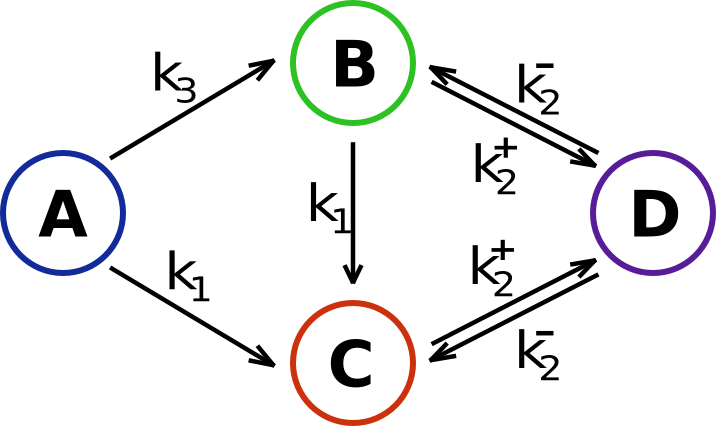
\includegraphics[width=15cm]{rxnNetwork}
  \caption{Graphical representation of a simple chemical reaction. The resulting network is weighted (by reaction constants), directed (based on reaction interactions) and labeled (by chemical formula).}
  \label{fig:rxnNetwork}
\end{figure}
\vspace{1mm}\\
There are many ways of specifying a graph, the simplest being a list of all $v_{i}$ and $e_{ij}$ present. However, the most popular method of description is through an ``adjacency matrix''. This is a square, $n \ \times \ n$, matrix in which $A_{ij}=e_{ij}$. This form is especially helpful when the underlying graph is undirected ($e_{ij}=e_{ji}$) as the adjacency matrix is symmetric. The degree of a vertex is an important measure of its connectedness in the graph, and is given by $d_{i}=\sum\limits_{i=0}^n e_{ij}$; thus, in an unweighted graph, the degree of a vertex is simply the number of edges connected to it (with loops counted twice). With this foundation, we continue with the original material.
%INCLUDE LATER An interesting property of the adjacency matrix is that the graph it represents is unchanged by permutation of its rows and columns. This is a result of working with unlabeled graphs, in which each vertex has the same ``identity''. Thus, if we consider the label of a vertex the it's row/column in the adjacency matrix, we can re-label it by switching it's row and column with that of another vertex, but the graph's structure remains unaffected. The significance of this fact will be detailed below.
\subsection{Network generation}
Significant effort has been spent researching algorithms that create networks with different properties. By far the most popular method creates what is called an Erd\H{o}s-R\'{e}nyi random graph. Proposed in 1959 \cite{originalERpaper}, it consists of the following simple procedure: given a set of vertices $V$ and a probability of connection $p$, examine each possible edge in the graph (note there are ${n \choose 2}$ possible edges in an undirected graph) and, with probability $p$, let $e_{ij}=e_{ji}=1$, otherwise $e_{ij}=e_{ij}=0$. Simply put, each edge exists with probability $p$. As previously mentioned, this straightforward method facilitates theoretical calculations \cite{a couple math papers}, but, as one might guess, few real-world systems follow such a simplistic scheme. The need for new algorithms was clear. \vspace{1mm}\\
To-date, many different methods of graph generation have been proposed. They largely fall into two categories: those which describe an evolution of the graph to its final state, and those which generate graphs with specified properties. A famous example of the former is the scale-free preferential attachment model \cite{emergenceOfScalingInRandNet}. The method is as follows: begin with a small number of disconnected vertices, $n_{0}$. Add a new vertex, and connect it to $m\le n_{0}$ of the pre-existing vertices. Let the probability that the new vertex, $v_{new}$, connects to one of the old vertices, $v_{old}$, be $P(e_{v_{new}v_{old}}=1)=\frac{d_{old}}{\sum\limits_{i} d_{i}}$. This method of attaching new edges leads to a rich-get-richer effect observed in many real-world situations. Note that no graph properties have been specified $a\ priori$ (except, trivially, the size $n$). In contrast, consider the Erd\H{o}s-R\'{e}nyi model just described. Here, the average degree, $\bar{d}$, is specified beforehand (this is equivalent to setting the probability of attachment, $p$, as then $p=\frac{n\bar{d}}{2 {n \choose 2}}$), and a graph is constructed to match this stipulation. While the method of evolving a graph to its final form is useful when this growth mechanism is understood, these models are specialized to the system under investigation. When information on the evolutionary process isn't available (as if often the case), it is more useful to measure certain features of the network in question, and use the property-specification class of methods to generate a graph with similar characteristics.\vspace{1mm}\\
The number of such methods, and the variety of properties addressed by them, has grown steadily in recent years. From efficient procedures generating Erd\H{o}s-R\'{e}nyi random graphs, to those that enable the simultaneous assignment of degree distribution and clustering coefficients \cite{efficentAlgsRG} \cite{the something somethig paper}, a wide range of variables are tunable in the current collection of methods. The shortcoming of all but one of the approaches in this toolset is that each deals with only a small number of specific properties. If the network under consideration has a certain degree distribution, and specific degree-triangle correlations, you must hope that an algorithm has been developed to deal exactly with the creation of a graph with a given degree distribution and degree-triangle correlation. One cannot simply take a method for degree distributions and combine it with a degree-triangle method to achieve the desired outcome. \vspace{1mm}\\
An innovative approach to this problem, the product of collaboration between the Floudas and Kevrekidis groups, aims to alleviate this hindrance. Their approach, detailed in \cite{karthiksOptim}, is to formulate the problem as a task for mixed-integer linear optimization. Using this optimization framework, they are able to add property specifications to the algorithm as needed. Each variable that needs to be addressed can be added as a building block in the overall formulation, tunable to the unique needs of each graph. Additionally, this method can guarantee the non-existence of certain graphs, a useful feature when detailing multiple complex properties. The downside of this wonderful generality is computational slowness. Searching the solution space of all possible graphs can become a daunting task at even modest sizes of $n=15$ if the searched-for graph is highly detailed. Using certain pre-processing steps, the speed has been greatly increased, but work remains if the method is to be applied to larger systems of $n>100$. 
%possibly remove
\begin{figure}[h!]
  \centering
  \includegraphics[width=15cm]{karthikOpt}
  \caption{Networks generated by the optimization framework presented in \cite{karthikopt}. The distribution of degrees is identical in both, but \ref{opta} exhibits high assortivity (vertices with large (small) degree link to others with large (small) degree), while \ref{optb} exhibits low assortivity.}
  \label{fig:rxnNetwork}
\end{figure}
\vspace{1mm}\\
Certainly, each algorithm has its unique strengths and weaknesses. While some can rapidly construct very large graphs ($n>100,000$), these have been created to address only a few of the many potentially interesting properties of a network. The one method that allows users to add properties as desired suffers from scalability issues. The efficient creation of networks with arbitrary property specifications remains an open area of investigation.
\subsection{Data Mining in Networks}
In the past decade, several factors have combined to fuel a wave of algorithms which aim to make sense of massive data sets. The internet has played no small role, as millions of users give information to online websites wittingly (through user accounts) or not (through cookies). Additionally, the proliferation of electronic sensors in everything from cars to refridgerators has given companies access to a far greater variety and quantity of information. Crucially, too, saptiotemporal resolution of research experiments has become increasingly commonplace. Here enter data mining techqniues, used to extract useful conclusions from such massive volumes of data. From the original workhorse, principal component analysis (PCA), useful in finding data embedded in linear subspaces, to new, nonlinear manifold learning techniques such as diffusion maps, today's techniques exhibit a wide range of approaches to dimensionality reduction \cite{data mining papers}. However, these methods are not currently well-suited for data mining across networks. Generally speaking, the goal of a data mining algorithm is to take a collection of points in $\mathbb{R}^{n}$, $n\gg1$ and embed it in $\mathbb{R}^{m}$, $m \ll n$, where the $m$ new dimensions capture the important details of the data. In many cases, data is easily amenable to such a description (e.g. a vector \textit{\{age, longitude, latitude\}} for Amazon users). Unfortunately, when each data point is, itself, a network, there is no clear way to initially ``pre-embed'' each point into $\mathbb{R}^{n}$, and thus the host of techniques proven in other applications become useless. The two options are then to develop new techniques that specifically address the unique aspects of network data, or to devise a scheme that adapts established techniques to operate on graphs (be it through some pre-embedding or otherwise). We focus on the latter approach. \vspace{1mm}\\
Many existing methods employ some measure of distance between points in their formulation. For example, a popular implementation of diffusion maps requires a weight matrix $W_{ij}=e^{-\frac{\|x_{i}-x_{j}\|^{2}}{\epsilon}}$, in which $x_{i}$ and $x_{j}$ are members of the dataset. This not always straightforward (e.g. if the data includes gender, a quantitative distance is unclear), but some (potentially weighted) \textit{\mathcal{p}-norm} is often suitable. Attempting to generalize vector or matrix norms might seem a natural place to start in defining distances between two graphs. As a norm, we would expect $\| x - y \| = 0 \Leftrightarrow x = y$. Unfortunately, even determining whether two graphs are equivalent is a complete research puzzle unto itself, and is termed ``the graph isomorphism problem''.
\subsubsection{Graph Similarity and Isomorphism}
%figures galore
To understand the issue at hand, we must first discuss the distinction between labelled and unlabelled graphs. A labelled graph is one in which the vertices have been assigned a unique identification. In the case of a transportation network of highways between cities, the city names could function as labels. Then, if, say, tasked with determining whether U.S. roadways changed between 1980 and 1981, simply checking whether each city's connections remained the same would suffice. The vertices of an unlabelled graph have no such intrinsic identity. Consider the popular epidemiological SIR model, in which vertices represent people and edges interactions between them by which diseases can be transmitted. Here, each node lacks information beyond the fact that it represents a single person. Comparing two networks is no longer so easy as checking whether all connections to and from each node are the same, as there is no way to identify a node from the first graph, $v_{old}$, with an equivalent node, $v_{new}$, in the second. To be sure two unlabelled graphs are, indeed, different, all possible pairings of nodes from graph one and two must be considered. This is the \textbf{NP} problem of determining graph isomorphism (whether two graphs can be labeled in such a way as two make their connections equivalent).
\begin{figure}[h!]
  \centering
  \includegraphics[width=15cm]{ismorphicGraphs}
  \caption{Despite appearing completely different, these graphs are equivalent to each other. Even in this tiny system, a brute force method of checking isomorphism would need to compare 'bell number' configurations.}
  \label{fig:isomorph}
\end{figure}
\vspace{1mm}\\
Given the inability to tell even whether two graphs are the same (in reasonable numerical time), the difficulties in defining a computationally tractable distance measure are understandable. Short of attempting a Clay Millenium Prize by proving \textbf{P}$ \ = \ $\textbf{NP}, one possibility is to accept an imperfect ismorphism method with guaranteed error bounds. Approximation algorithms do exist for this problem, but they have yet to be applied in this context. The hope would be to extend one of these to output some indication of the differences between graphs (and not just a boolean judgement of ismorphism), and to use this modified method as the requisite distance measure in pre-existing data mining routines. The application of such techniques to sets of graphs would be a novel and beneficial step in the analysis of these datasets.
%I think your original example about religions is flawed, that's data in a network, unless you want to include that as a possible area of research
\subsection{Accelerated Network Simulations}
Real-world networks are often many-membered ($n>10,000$) and frequently exhibit complex dynamics between nodes (e.g. a differential equation describing a flow along an edge). Developing accurate models is a challenge in itself, but even when available, simulating such large, sophisticated networks is computationally prohibitive. As mentioned above, the time required to reach a system's steady-state is, in a number of cases, a function of the problem size \cite{votingmodel1} \cite{votingmodel2} \cite{prefattach}. Thus, both storage space and simulation length increase with $n$. A method of accelerating such laborious calculations would be highly valuable. Coarse projective integration schemes could enable such a speedup, but this would require a good macroscopic description of the network, along with some method of translating these macroscopic variables into realizations of a microscopic system. Advances in the previous two sections would allow for both.\vspace{1mm}\\
Coarse projective integration (CPI) exploits the separation of timescales inherent in many systems to expedite simulations. The framework is very general, and has been successfully applied to many systems \cite{cpi papers}. There are two prerequisites: that there exist a small number of good, coarse variables that adaquately describe the system (but for which closed equations or models are not available), and that, given certain macroscopic property specifications, a microscopic system can be created that contains these characteristics. A CPI method can then be implemented using the following general outline: first, detailed, microscopic simulations are initialized, and the selected coarse variables are periodically calculated as the system evolves. Given this evolution of coarse variables, one then projects the system forward in the low-dimensional space to obtain new macroscopic values. Finally, these new variables are used to restart full microscopic simulations, at which point the process can be iterated until the desired state is reached. \vspace{1mm}\\
CPI has already been applied to evolving networks, but these implementations have depended on two things. First, that suitable coarse variables could be discerned from careful observation of the system, and second, that there existed an algorithm to generate graphs with such values \cite{bold and karthik} \cite{kathik prl}. Demonstrating that either a data mining algorithm can be employed to find such coarse variables or that a generic network generator can initialize the necessary microscopic simulations would significantly generalize the CPI approach for use in a wider variety of network problems. \vspace{1mm}\\
However, CPI is but one member of a suite of methods that analyze coarse-grained systems. Coarse fixed point computations are possible by solving $f(x) - \Phi_{t} (x) = 0$ for $x$, where $f(x)$ is the macroscopic function evolving to a fixed point, $x$ represents the system's state, and $\Phi_{t} (x)$ is the function's value after being projected forward (in the low-dimensional space) a length $t$. While the derivatives of $\Phi_{t} (x)$ are typically needed, they can be estimated numerically \cite{bold}.  The conjugate gradient method can also be implemented on a coarse level to expedite searches for minima. Consequently, successes in network generation and data mining algorithms open the door to an array of analytical techniques. Combining these disparate methods (network generation and dimensionality reduction) would be the ideal culmination of this work. \\ \\
Graph generation, detection of signficant features across networks, and accelerated simulation of such complex systems are each interesting avenues of research in their own right. It is hoped that the synthesis of these three elements will allow researchers to more accurately model real-world networks, attain useful information from such models, and simulate full-scale systems in reasonable computational times.
\section{Current Work}
Initial research has focused on accelerating simulations of dynamical network systems. While leaping to the third of three steps may seem premature, it quickly reveals weaknesses in the overall process of simulation, and serves as a guide for future investigation. Two cases were studied, a voting model with possible applications in sociology, and an edge reconnecting model, which mainly serves as a toy mathematical network for which behavior can be derived theoretically. After briefly describing the dynamics of each, current progress in simulation acceleration will be discussed.

\subsection{Voting Model}
The \textit{k} opinion voter model initally consists of an Erd\H{o}s-R\'{e}nyi graph of size $n \ (>10,000)$, with small average degree ($\bar{d}\asymp 1$). To begin, each vertex is randomly assigned an opinion based on some initial distribution $\{p_{i}\}_{i=1}^{k}$. With this initial state and a ``probability of reattachment'' $\alpha$, the graph evolves as follows (note that $\zeta(v_{i})$ denotes the opinion of $v_{i}$):
\begin{enumerate}
\item Choose an edge $e_{ij}$ uniformly at random from $E(G)$
\item Randomly choose one of the endpoints of $e_{ij}$, call it $v_{i}$ (the other endpoint will be $v_{j}$)
\item Repeat steps one and two until $\zeta(v_{i}) = \zeta(v_{j})$, i.e. the vertices' opinions do not match
\item With probability $\alpha$, remove $e_{ij}$ from the graph
\begin{enumerate}
\item Choose a new vertex $v_{k}$ uniformly at random from $V(G)$ until $e_{ik} \notin E(G)$ 
\item Add $e_{ik}$ to $E(G)$
\end{enumerate}
\item Otherwise (with probability $1-\alpha$), set $\zeta(v_{i}) = \zeta(v_{j})$
\end{enumerate}
This process is iterated until the system reaches a consensus state in which $\zeta(v_{i}) = \zeta(v_{j}) \forall v_{i}, v_{j} \in V(G)$, i.e. every edge connects vertices of the same opinion. An edge $e_{ij}$ is called a conflict whenever $\zeta(v_{i}) \ne \zeta(v_{j})$. Thus the system is evolved until all conflicts are removed. While the general \textit{k} opinion model has received some attention \cite{durretts preprint?}, our focus will be the simpler two opinions (0 and 1). In this case, it has been shown that, for a certain initial minority fraction $p_{minority} \le 0.5$, a bifurcation occurs as $\alpha$ increases. At low values of $\alpha$, fewer edges are rewired and the system approaches a static state. In this limit, the system should converge approximately once each of the $m$ edges are selected, which occurs in $O(n\sqrt{n})$ steps (according to results from what is known as the coupon collector's problem) \cite{durrett}. As $\alpha$ increases, so does the frequency of rewiring. This slows the rate of consensus to $O(n^{2})$. Interestingly, besides differences in convergence speed, the final consensus state also changes. In the low-$\alpha$ limit, the final minority fraction is an increasing function of $\alpha$. In the slower, high-$\alpha$ range, the final minority fraction is unchanged from the initial value. Fig. \ref{biffig} illustrates the effect of $\alpha$ and $p_{minority}$ on the final consensus state.\vspace{1mm}\\
By creating phase plots of different system properties (e.g. minority fraction, number of conflicts), it was observed that the minority fraction dictates the state of the system. Fig. \ref{durrett's figures of minority fractions} shows how both the number of conflicts and the number of connected vertex triplets with two vertices of opinion 0, and one of 1, could be written as functions of the minority fraction. This suggested that the system minority fraction could serve as a macroscopic variable in CPI. The system is stochastic, so in order to obtain smooth evolutions of variables the average trajectory of an ensemble of voting models is used. In fact, both the minority fraction and conflict count were used as coarse variables (though conflict count appears slaved to minority fraction is likely unecessary). After projecting these variables forward in macroscopic space, the graph generation problem must be addressed. Thankfully, creating a network with a certain minority fraction and conflict number is a simple task, and a customized algorithm was developed. CPI results are shown in Fig. \ref{voting model cpi}. This CPI implementation reduced the number of microscopic steps needed to reach consensus by an average of 50\%.

\subsection{Edge Reconnecting Model}
The edge reconnecting model, proposed in \cite{balazs'paper}, presents special difficulties in creating accurate low dimensional representations of the overall system. Namely, the network is allowed to have multiple edges connecting the same vertices (such a construction is termed a ``multigraph''). Initially, $m\asymp n^{2}$ edges are distributed uniformly among the $n$ vertices. Then the multigraph evolves as a Markov chain according to the following dynamics:
\begin{enumerate}
\item Choose an edge $e_{ij} \in E(G)$ uniformly at random and flip a coin to label one of the ends as $v_{i}$
\item Choose a vertex $v_{k}$ using linear preferential attachment: $P(v_{k} = v_{l}) = \frac{d_{l}}{\sum\limits_{i=1}^{n} d_{i}}$
\item Replace $e_{ij}$ with $e_{ik}$
\end{enumerate}
This process is repeated until a frozen state is reached, at which point the degree distribution ceases to change.\vspace{1mm}\\
Interestingly, while the network is strictly unlabelled, the preferential attachment dynamics tend to stratify the vertices into a low degree majority and extremely high degree minority. This permits a sort of pseudo labelling of the vertices, as a vertex of high (low) degree at time $t_{1}$ is likely to retain its high (low) degree at $t_{2}$. Therefore, when sorted by degree, the evolution of the adjacency matrix appears smooth. \vspace{1mm}\\
Two distinct timescales arise from these dynamics, $T\asymp n^{2}$ and $T\asymp n^{3}$ where $T$ is the number of steps. On the faster, $O(n^{2})$ scale, the degrees of the vertices may be considered constant, while the number of parallel edges between vertices changes. On the slower $O(n^{3})$ scale, the degree distribution evolves to a steady state value. While this separation of timescales has been proven in \cite{balazs:rsa12}, identifying them through numerical simulations is complicated by a couple of factors. First, the exact timescales themselves are difficult to discern. Both scales are really $O(\rho_{1} n^{2})$ and $O(\rho_{2} n^{3})$, where the constants $\rho_{i}$ are evaluated at the limit of infinite-sized graphs ($n\rightarrow \infty$). This hints at the second, larger, problem: many of the results on the existence of these timescales in the first place are only valid in this large-$n$ limit. Simulation time then becomes problematic. Figs. \ref{fig:nSquaredTimescale} and \ref{fig:nCubedTimescale} illustrate attempts to visualize these separate scales of evolution. The degree distribution is plotted every $n^{2}$ steps in the figures, with a total number of $n^{3}$ steps in each. The changes appear quite gradual, and no distinct timescales are evident.\\
%insert figure
Our approach in coarse-graining system dynamics is based on the existence of a gap in the spectrum of the adjacency matrix, and the subsequent ability to approximate $A\approx \lambda_{1}v^{(1)}v^{(1) \;\dagger}$ where $A$ is the adjacency matrix of the system, $\lambda_{1}$ is the leading eigenvalue of $A$, and $v^{(1)}$ the corresponding eigenvector. Fig. \ref{fig:spectralGap} shows that clearly $|\lambda_{1}| \gg |\lambda_{i}|, i=2,3,...,n$. \\
Fig. \ref{fig:adjRecon} illustrates the reconstruction of the adjacency matrix as $A_{ij}=\lambda_{1}v^{(1)}_{i}v^{(1) \;\dagger}_{j}$ (after multiplication, each entry $A_{ij}$ was rounded to the nearest integer if $i\neq j$ or to the nearest even integer if $i=j$). Visually, the two correspond very well. \\
As $\lambda_{1}v^{(1)}v^{(1) \;\dagger}$ appears a good approximation of $A$, it was reasoned that we could use this eigenvalue/eigenvector combination as a coarse description of the system. In order to further reduce dimensionality, the eigenvector was fitted with a fifth-degree polynomial, as shown in Fig. \ref{fig:eigVectFitting} (a fifth-degree polynomial was used as additional terms didn't significantly increase fitting accuracy). The six coefficients of this function were then used as a smaller set of coarse variables, leading to a final seven-dimensional representation of the system (six coefficients plus an eigenvalue). The following outlines the CPI framework:
\begin{enumerate}
\item Simulate the full edge reconnecting model dynamics for some number of steps until the fast variables are sufficiently slaved to the slow
\item Record the adjacency matrix as the system evolves on the slow manifold (in fact, it is more efficient to immediately compute the leading eigenvector, fit it with a polynomial, and store only these coefficients, along with the leading eigenvalue, as time progresses)
\item Project forward the coarse variables (coefficients and eigenvalue)
\item Reconstruct a new adjacency matrix from the new, projected coefficients and eigenvalue:
  \begin{enumerate}
  \item Compute a new eigenvector as $v(i) = \displaystyle\sum\limits_{k=0}^{k=6} i^{k}c_{k}$ (where $c_{k}$ represents the coefficients of the polynomial and $v(i)$ the $i^{th}$ component of $v$) and round to the nearest integer
  \item Compute the new adjacency matrix as $A_{ij}=\lambda_{1}v^{(1)}_{i}v^{(1) \;\dagger}_{j}$ and round as discussed previously
  \end{enumerate}
\item Repeat step one until system reaches steady state
\end{enumerate}
Preliminary results of this method are shown in Fig. \ref{fig:CPI}, in which the evolution of the degree distribution is shown for both the full simulation and a simulation in which CPI has been employed. On average, CPI required 50\% fewer steps than the full simulation to converge to a fixed point.
\section{Recent Advances in Literature}
Graph Kernels\\
Coarse MD simulations\\
\section{Future Work}
A number of areas present themselves as good research directions. They're divided by subject below.
\subsection{Graph Generation}
The recent optimization based method of graph generation will certainly serve as a starting point for this avenue. The main limitation of the approach its scalability. Preprocessors have been shown to significantly reduce runtimes, but have been created to address specific properties. These operate by removing search paths unlikely to yield the specified graph before the optimization algorithm begins. This works particularly well when many distinct (non-isomorphic) graphs exist that satisfy the stipulations. In this case, the preprocessor does not need to be particularly careful in its deletions, as it is unlikely to remove all branches leading to feasible solutions. When more specificity is needed, it is possible to tune this step to be more cautious in its selections. Creating a generic preprocessor for arbitrary properties would retain the generality of the method while increasing speed. \\
\subsection{Data Mining across Graphs}
This nascent research topic hasn't received much attention yet. Certain sub-problems (graph isomorphism, vertex matching) have been thoroughly investigated, but the concept of applying dimensionality techniques when data points are, themselves, networks seems new. As mentioned, it may be possible to adapt an existing approximation algorithm that determines graph isomorphism to additionally yield information on the differences between two networks. A thorough understanding of the structure of these methods through an extensive literature review will be a necessary starting point. \vspace{1mm}\\
The little related work that has been done involves defining kernels over graphs \cite{graph kernels}. These all seem to be based on random walks over the network, and subsequent comparisons of the traversed paths. By defining a measure of similarity between two paths, the collection of walks over each graph can be compared to find a similarity of the graphs as a whole. It would be interesting to investigate the possible relationships between these methods and diffusion maps, which appear to have been formulated independently. Otherwise, the foundation of these graph kernels, a paper from 1999 \cite{hausler}, provides a general framework from which other kernels could be invented. \vspace{1mm}\\
In general, work would focus on developing graph similarity measures in simple models, such as Erd\H{o}s-R\'{e}nyi, in which issues would be more readily diagnosed and guarantees of success or failure more easily proven. Additionally, simpler, heuristic measures of graph similarity have been shown to work in certain scenarios \cite{karthik secondprop}. These could be used while more grounded methods are developed, or a combination of simple measures could be found that adequately addresses our needs.
\subsection{Coarse System Dynamics}
The immediate aim in this direction will be to apply diffusion maps to the voting model data in an attempt to recover the minority fraction as a good coarse variable. This is expected to work, as DMAPS has been able to discover appropriate coarse variables in other collections of graphs using heuristic similarity measures. It may be difficult to implement a coarse fixed point method on the system, as the final system state is artificial. Unlike a tradional steady state, a voting model simulation ends not when it ceases to change with time, but when all conflicts are resolved. If the system were left running, it would not necessarily remain in the same configuration. Outside of the voting and edge reconnecting models, the search will continue for systems with separations of timescales amenable to coarse analysis.\vspace{1mm}\\

%\bibliographystyle{abbrv}
%\bibliography{firstprop_bib.bib}
\end{document}
